\documentclass[11pt,a4paper,twoside]{memoir} 

\usepackage[spanish]{babel}

\usepackage[bookmarks=true]{hyperref}

% Agrega toc al toc
\usepackage{tocbibind}

\usepackage[acronym]{glossaries}
\makeglossaries

\newacronym{si}{SI}{Sistema Informático}

\newacronym{osu}{OSU}{Obra Social Universitaria}

\newacronym{dospu}{DOSPU}{Dirección de Obra Social para el Personal Universitario}

\newacronym{decom}{DECOM}{Departamento de Complementación}

\newacronym{fesac}{FESAC}{Fondo Especial Solidario para Alta Complejidad}

\newacronym{sumas}{SUMAS}{Sistema Universitario Médico Asistencial Solidario}

\newacronym{unsl}{UNSL}{Universidad Nacional de San Luis}

\newacronym{cmmu}{CMMU}{Cuota Mensual Máxima Única}

\newacronym[
	description={Decision Requirements Diagram}
]{drd}{DRD}{Diagrama de Requemientos de Decisión}

\newacronym[
	description={Drools Rule Language}
]{drl}{DRL}{Lenguaje de Reglas de Drools}

\newacronym[
	description={Friendly Enough Expression Language}
]{feel}{FEEL}{Lenguaje de Expresión Suficientemente Amigable}

\newacronym[
	description={Decision Model Notation}
]{dmn}{DMN}{Notación de Modelo de Decisión}

\newacronym[
	description={Plain Old Java Object}
]{pojo}{POJO}{Objeto Java Simple}



\usepackage[inline]{enumitem}

\usepackage{caption}
\captionsetup[listing]{name=Listado}

\usepackage{cleveref}
\crefname{listing}{listado}{listados}
\Crefname{listing}{Listado}{Listados}

\usepackage{fontspec}
\setmonofont{MesloLGS NF}

\usepackage[]{minted}
\setminted[]{
    breaklines,
    breakafter=(.,
    fontsize=\scriptsize,
    linenos,
    escapeinside=||,
    frame=single,
    rulecolor=\color{black},
    tabsize=2,
}
\setmintedinline[]{
    fontsize=\scriptsize,
}

\usepackage{graphicx}
\graphicspath{ {./images/} }

\usepackage{csquotes}
\usepackage[backend=biber, style=numeric, sorting=none, bibstyle=alphabetic, maxnames=10, minnames=6,backref=true, autocite=inline, labelalpha=true, doi=false, url=false]{biblatex}
\addbibresource{the.bib}
% tablas
\usepackage[margin=1in]{geometry}
\usepackage[table,dvipsnames]{xcolor} 
\usepackage{multirow}
\usepackage{etoolbox}
\usepackage{tabularx}
\usepackage{array}
\newcolumntype{C}[1]{>{\centering\arraybackslash}p{#1}}

% Use more than one optional parameter in a new commands
\usepackage{xargs}                      

\usepackage[spanish,colorinlistoftodos,prependcaption,textsize=tiny]{todonotes}
\newcommandx{\desarrollar}[2][1=]{\todo[linecolor=blue,backgroundcolor=blue!25,bordercolor=blue,#1]{#2}}
\newcommandx{\modificar}[2][1=]{\todo[linecolor=Plum,backgroundcolor=Plum!25,bordercolor=Plum,#1]{#2}}
% \newcommandx{\unsure}[2][1=]{\todo[linecolor=red,backgroundcolor=red!25,bordercolor=red,#1]{#2}}
% \newcommandx{\info}[2][1=]{\todo[linecolor=OliveGreen,backgroundcolor=OliveGreen!25,bordercolor=OliveGreen,#1]{#2}}
% \newcommandx{\improvement}[2][1=]{\todo[linecolor=Plum,backgroundcolor=Plum!25,bordercolor=Plum,#1]{#2}}
% \newcommandx{\thiswillnotshow}[2][1=]{\todo[disable,#1]{#2}}


\newcommand{\SIOSU}{\acrshort{si}--\acrshort{osu}}

\newcommand*{\thistitle}{\begingroup% based on titleJT
	\centering
	{\huge\bfseries Informe: Práctivas Profesionales\par}
	\vspace{1.5cm}
	{\Large Estudiante: Iván Brocas\par}
	\vspace{0.7cm}
	{\Large N° de Registro: 3027820\par}
	\vspace{0.7cm}
	{\Large\itshape Carrera: Ingeniería en Informática\par}
	\vspace{1.5cm}
	{\scshape\LARGE Universidad Nacional de San Luis\par}
	\vspace{1cm}
	
\includegraphics[width=0.35\textwidth]{logo-UNSL}\par\vspace{1cm}
	\vspace{0.5cm}
	{\scshape\LARGE Dirección de Obra Social para el Personal Universitario\par}
	\vspace{1cm}
	
\includegraphics[width=0.35\textwidth]{logo-DOSPU.jpg}\par\vspace{1cm}
	\vfill
	\endgroup}

\newcommand{\code}[1]{{\small\texttt{#1}}}

\let\originalacrfull\acrfull
\RenewDocumentCommand{\acrfull}{m}{%
  \ifglshasfield{user1}{#1}{%
    \glsentrylong{#1} (\glsentryuseri{#1}, \glsentryshort{#1})%
  }{%
    \originalacrfull{#1}%
  }%
}


\title{Informe PPS}
\author{Iván Brocas}

\begin{document}

% \thistitle

% Esta lista se borra al momento de distribuir
% \cleardoublepage
% \listoftodos
% \todototoc

% \cleardoublepage
% \chapter*{Resumen}

% \cleardoublepage
%  \renewcommand{\contentsname}{Tabla de contenidos}
% \tableofcontents

\printglossary[type=\acronymtype]

% 8. Selección de caso puntual para prototipar la separación de las reglas de cálculo del
% código fuente
% 9. Implementación de tests de verificación de correcto comportamiento de la aplicación
% para el caso puntual.
% 10. Implementación del cálculo para un caso puntual y verificación del correcto
% comportamiento.

\chapter{Introducción}

\modificar[inline]{Revisar, modificar y ubicar cada uno según creas conveniente.}

Este proyecto plantea avanzar hacia SIOSU-Moambue, un sistema informático (SI) para obras sociales universitarias (OSU) con características ágiles y de centricidad en el afiliado. La agilidad procura facilitar la evolución en respuesta a cambios y la adaptación/adopción por distintas OSU del país a un costo accesible.  La centricidad en el afiliado (paciente) es la característica preponderante en las innovaciones introducidas recientemente en los sistemas informáticos de salud a partir de avances en distintas tecnologías (Salud 4.0).

El SI de una OSU debe mantenerse “vivo”. Su utilidad, el valor que genera su funcionamiento, disminuye conforme pierde sintonía con los cambios que tanto la organización (por ejemplo, cambios en políticas y reglamentos locales) como su contexto sufren (como ser, cambios en leyes nacionales y provinciales, situaciones sociales o económicas a las que se debe atender, o eventos como Covid-19). Dado que el cambio es la norma, no la excepción, la sistemática falta de evolución de un SIOSU representa su agonía y eventual muerte, e innumerables perjuicios para la OSU y sus afiliados. Inicialmente los funcionarios adaptan sus procesos de trabajo para responder a las modificaciones (posiblemente usando planillas electrónicas o papel), incrementando sistemáticamente la parte manual del trámite en detrimento de la automática. Conforme el estado agónico se profundiza, los funcionarios comienzan a verse abrumados por el trabajo y perciben poco práctico usar las funcionalidades desactualizadas del SIOSU; los trámites que podrían resolverse en minutos, comienzan a llevar horas, días o meses.  Además, los responsables de la gestión experimentan la falta de información actualizada para respaldar sus decisiones, las cuales en ocasiones no pueden demorarse debido a la necesidad de responder a proveedores y prestadores de servicios que podrían interrumpir sus servicios. Por otro lado, el descontento entre los afiliados crece;  perciben que sus trámites no avanzan; que no tienen respuestas por parte de los funcionarios, pero estos a su vez no disponen del tiempo y posiblemente tampoco de las funcionalidades correctas del SIOSU para hacerlo. 

También debe ser tenida en cuenta la revolución innovadora Salud 4.0. Esta se enmarca en la guía de Objetivos de Desarrollo Sostenibles 2030 planteada por la ONU, cuyo tercer objetivo es justamente “Salud y Bienestar”. En general, se busca introducir cambios políticos, económicos, sociales y culturales en diversas esferas de la vida y actividad humana que representen avances catalizadores del progreso y transformación digital de la economía, de los sistemas de producción y de la mejora de la calidad de vida de la sociedad y su respeto a los ecosistemas. En particular, Salud 4.0 nuclea las innovaciones que buscan centrarse en el paciente (impulsadas principalmente por COVID-19) de manera de brindar una atención personalizada que facilite, por ejemplo, detectar anticipadamente y prevenir patologías. Estas innovaciones las posibilitan principalmente los avances en el tratamiento masivo de datos, la ciencia de datos, la inteligencia artificial, los sistemas ciber-físicos, la computación en la nube, y los dispositivos móviles. 

Sin duda es conveniente para las OSU adoptar estas innovaciones. No solo permiten cuidar mejor la salud de sus afiliados y prevenir procedimientos riesgosos y costosos, sino que también se evitan visitas innecesarias a oficinas. De esta manera, se logra la reducción de  costos operativos y se mejoran las posibilidades de inversiones futuras que produzcan  mejoras más profundas en la atención a los afiliados.

Sin embargo, a pesar de los beneficios mencionados, las OSUs difícilmente evitan que sus SIs entren en agonía y en general no abordan innovaciones Salud 4.0 (las cuales son únicamente adoptadas por selectos proveedores de salud privada, muchas veces inaccesible para la población general). Las opciones que tienen las OSU para sacar a sus SIs del camino de la agonía pueden, en general, clasificarse en tres: (a) incorporar/escalar su propia área de informática de manera que esté a la altura del desarrollo y mantenimiento de software necesarios; (b) contratar a una empresa para que esté a cargo de este desarrollo y mantenimiento; y (c) comprarle a una empresa el producto ya desarrollado y pagar por su adaptación y mantenimiento. Es preciso señalar en este punto que las opciones (a) y (b) implican que la OSU sea propietaria del sistema que quieren revitalizar. También se debe estudiar con mucho cuidado la opción (c), el reemplazo del sistema agonizante por uno propietario “enlatado”, que a primera vista puede parecer la opción menos onerosa y más rápida de concretar. La realidad de las OSU es notablemente más compleja que la de las obras sociales privadas. Sus afiliados tienen mayor poder de decisión, muchas veces a través de asambleas. Esto hace que los tipos de afiliados, las reglas de negocio, y los planes de salud sean más equitativos, pero a su vez más complejos. La complejidad también es mayor en la gestión de convenios con prestadores. Al tener un volumen de afiliados reducido, la OSU debe negociar convenios más detallados y asumir la complejidad que las organizaciones prestadoras impongan. Para llevar adelante la opción (c) se deberá pagar la licencia del SI, y luego meses de desarrollo para poder adaptar el mismo a las reglas de negocio de la OSU. Una vez puesto en producción, se deberá conservar la relación con la empresa proveedora, abonando diariamente el mantenimiento y evolución del SI. Además, si se tiene en cuenta que la exportación de servicios informáticos de Argentina representa el 9\% de las exportaciones de servicios, y que los profesionales con la capacidad de llevar adelante el desarrollo necesario, en general cotizan su trabajo a valor dólar, es posible entender que cualquiera de las opciones se tornan inviables para las OSU de menor envergadura, y difíciles de llevar adelante para las de mayor volumen de afiliados, pudiendo incluso no lograr responder a las necesidades de cambio a pesar de las erogaciones y esfuerzo realizados.

La Dirección de Obra Social para el Personal Universitario (DOSPU) de la UNSL no escapa a este problema. La presidencia de DOSPU, el Rectorado, la Facultad de Ciencias Físico-Matemáticas y Naturales, y su Departamento de Informática se encuentran colaborando para reemplazar su antiguo SI que agoniza, y en el proceso causa perjuicios – como los antes enumerados – a la organización. El nuevo sistema, SI-DOSPU, está siendo desarrollado usando prácticas de las metodologías ágiles (scrum, product discovery, behaviour driven development, test driven development, e integración y despliegue contínuo) y sobre  tecnologías de punta incluyendo las que posibilitan desplegar en proveedores de computación en la nube. Este esfuerzo se ha dividido en tres etapas con los siguientes objetivos: (1) reemplazar el antiguo SI y automatizar procesos; (2) dar soporte a la toma de decisiones de la gestión a partir de la creación de un repositorio para el análisis de información y extracción de conocimiento; (3) introducir mejoras en los procesos con el objetivo de centrarlos en los afiliados. Actualmente SI-DOSPU se encuentra en su etapa (1) con la mayor parte de la funcionalidad implementada y en un proceso de carga de datos previos a la puesta en producción. Cabe destacar que el mayor inconveniente que se ha encontrado en el desarrollo de la etapa (1) radica en la resistencia cultural al cambio, a pesar del escaso valor que proporciona el sistema agonizante y gran esfuerzo adicional que esto implica para los funcionarios.

SIOSU-Moambue se desarrollará a partir de SI-DOSPU y la experiencia ganada en su producción. Las OSU difieren en las políticas y reglamentaciones locales, pero es de esperarse que compartan gran parte de su conceptualización y mecanismos de trabajo. SIOSU-Moambue se desarrollará separando las reglas de negocio dependientes de políticas y reglamentaciones locales de manera de hacerlas flexibles y fácilmente modificables. El sistema será liberado con licencia open source y la OSU que quisiera adoptarlo deberá afrontar los gastos de adaptación y mantenimiento locales. Vale la pena destacar que se ha elegido la palabra guaraní “Moambue” que significa cambiar, ya que el foco de la iniciativa es que las OSU puedan evolucionar de manera ágil su SI para responder a los cambios a costos accesibles.

\section{Motivación}

\desarrollar[inline]{En esta sección, explicar el problema que enfrenta la organización al tener reglas complejas: muchas categorías, resoluciones con condiciones a contemplar. Y por otro lado, economía y condiciones sociales inestables.}

Durante su existencia, cada \acrfull{osu}, al igual que tantos otros tipos de organizaciones, se ve afectada por una plétora de cambios, que pueden ser tanto internos (por ejemplo, cambios en políticas y reglamentos), como en su entorno (como ser, cambios en leyes nacionales y provinciales, situaciones sociales o económicas a las que se debe atender, o eventos como Covid-19).
Indiferentemente de la naturaleza de dichos cambios, un \acrfull{si} que fallé en adaptarse a los mismos estará destinado a la obsolencia y eventual muerte, que suele ser precedida por un proceso de degradación del mismo.
Los usuarios del \SIOSU se ven obligados a suplir las funciones desactualizadas con trabajo manual (posiblemente haciendo uso de planillas electrónicas o papel), deshaciendo la automatización y degradando la eficiencia conforme los nuevos requerimientos se separan de aquellos para los que el sistema fue disñado.
Esto, a su vez, conlleva en un aumento de los tiempos requeridos para la realización de los trámites de la \acrshort{osu}, con los subsecuentes decrementos en la calidad del servicio prestado y la conformidad de los afiliados. Adicionalmente, la información se dispersa en los medios introducidos (planillas electrónicas o papel, por ejemplos), dificultando la recolección de información para el respaldo de decisiones.

Esta situación no es más que exacerbada en el caso de que la obra social cuente con reducido o carezca de personal técnico, capaz de trabajar para mantener el sistema consistente con la realidad.

Por otra parte, en el caso de que sea posible realizar los cambios necesarios al sistema, dichos cambios suelen requerir un re-despliegue del sistema, resultando en una menor disponibilidad del mismo. Esto resulta particularmente ineficiente en escenarios donde puede haber frecuentes cambios pequeños.

\section{Objetivo general}
Parametrizar el \SIOSU de \acrfull{dospu}, separando de las reglas de negocio de una obra social en particular del \acrshort{si}, utilizando para la escritura de las mismas un lenguaje inteligible para el personal de la obra social. Más concretamente, el alcance de este trabajo abarca la extracción de las reglas utilizadas para el cálculo de las cuotas de los afiliados.

Esto con el fin de facilitar, que los cambios puedan ser realizados por personal que no tenga conocimientos del funcionamiento interno del \acrshort{si}, facilitando la actualización de las reglas y permitiendo la reducción en la incidencia a o posiblemente una solución a los problemas mencionados.

\section{Objetivos específicos}
\begin{itemize}
	\item Extraer las reglas de negocios del código del \acrlong{si}.
	\item Expresar dichas reglas en un lenguaje que resulte entendible para el personal de la \acrlong{osu}
	\item Permitir la gestión de las reglas de forma independiente del \acrshort{si}.
	\item Reducir la cantidad de esfuerzo requerido para realizar cambios en las reglas.
\end{itemize}

\section{Enfoque adoptado}

\desarrollar[inline]{
    En esta sección explicas los pasos que seguiste, sin entrar en detalles.
    Debe quedar claro: 
    la (auto) capacitación (temas nuevos),
    el trabajo de análisis necesario,
    como se asegura la calidad, y 
    te debe dar la base para explicar en capítulo se desarrolla cada paso.
    }

\section{Organización}

\desarrollar[inline]{Breve descripción de lo tratado por cada capítulo}

Este informe está dividido en los siguientes capítulos:
\begin{itemize}
	\item Gestión de afiliados
	\item Revisión literia
\end{itemize}


\chapter{Estructura Organizacional \acrshort{dospu}}


\chapter{Categorías y cuotas de afiliación}

% Acá va el caso de estudio (la gestión de afiliados de DOSPU) 
% del cual se desprenden los requerimientos de expresividad para el motor de reglas

% En esta sección explicamos que los docentes y no docentes universitarios acceden a DOSPU por trabajar en la UNSL, pero que exiten otras formas de ingresar a la obra social. Es por esto que existen distintos tipos de afiliación y en los casos en que no están activos y se descuente por haberes, se debe calcular y cobrar su cuota, habiendo múltiples parámetros y reglas para esto. 
% En esta sección deben quedar en claro las categorías básicas de afiliados y que el cálculo de la cuota es complejo.
% Para el resto del capítulo basarse en el documento "DOSPU Afiliaciones y Cuotas" en google drive.

\section{Introducción}
Según lo establecido en \cite{dospuOrd53}, además del personal docente y no docente de la \acrfull{unsl}, otras personas que cumplan con las condiciones dictadas también pueden afiliarse a \acrshort{dospu}.

A raíz de esto, los afiliados se encuentran dividos en las categorías titular (\cref{sec:titular}), familiar (\cref{sec:familiar}) y voluntario adherente (\cref{sec:adherente}). Asimismo cada categoría está dividida en subcategorías, cada una utilizando distintas fórmulas o coeficientes en las mismas para el cálculo del aporte del afiliado.

\section{Titular} \label{sec:titular}

\subsection{Subcategoria: Obligatorio activo}
\begin{displayquote}
Agentes que se encuentren en actividad.
\hfill\parencite{dospuOrd53}, art. 24.1.A.
\end{displayquote}

Actualmente, este descuento no es cálculado por el \acrshort{si}, con lo cual está fuera del alcance de este trabajo.

\subsection{Subcategoria: Voluntario jubilado}
\begin{displayquote}
Agentes que al momento de pasar al régimen pasivo, eran afiliados obligatorios activos y
que opten voluntariamente, mediante formal solicitud por continuar perteneciendo sin
interrupción de aportes a esta Obra Social. La solicitud de afiliación debe ser solicitada en
un término no mayor de sesenta (60) días corridos a partir del cese de sus actividades. \hfill\parencite{dospuOrd53}, art. 24.1.B. 
\end{displayquote}

Monto de la cuota (\cite{dospuRes21} art. 2 y Anexo I): $$0.02 * j_m + 0.05 * j_h$$

, donde:
\begin{itemize}
    \item $j_m = \text{jubilación mínima}$
    \item $j_h = \text{haber jubilatorio}$
\end{itemize}

\section{Familiar} \label{sec:familiar}
\begin{displayquote}
\emph{No aportantes o eximidos de aportes}: El cónyuge, los hijos hasta la mayoría de edad establecida por el Código Civil vigente en la República Argentina, o que cursen estudios regulares hasta los 26 años y aquellas personas que pertenezcan al grupo de familiares primarios y están eximidos de aportar por disposición estatutaria o por Resolución de Directorio. No rige límite de edad para aquellos hijos discapacitados mientras dure su incapacidad.
\hfill\parencite{dospuOrd53}, art. 23.c.
\end{displayquote}

\begin{displayquote}
Familiares primarios de los titulares.
\hfill\parencite{dospuOrd53} art. 24.2.
\end{displayquote}

Distinto es el caso para cónyuges y convivientes de voluntarios jubilados, cuya cuota es un 70 \% de la del afiliado titular (\cite{dospuRes21} art. 2 y Anexo I).

% TODO: descuento en el caso de que ambos conyuges sean titulares.

\section{Voluntario adherente} \label{sec:adherente}
\begin{displayquote}
Son aquellos afiliados voluntarios que reúnen los requisitos establecidos en esta Carta Orgánica para ser incorporados a la Obra Social, siendo el Directorio de D.O.S.P.U. quien tiene a su cargo el dictado de las normas de afiliación, pagos de aportes y prestación de servicios correspondiente a cada categoría descrita en esta Carta Orgánica. En todos los casos y para concluir el trámite de afiliación en esta categoría, será requisito la presentación de garantía suficiente en resguardo del pago del aporte correspondiente. Además el Directorio de D.O.S.P.U. reglamentará un cálculo del aporte correspondiente por categoría con valores diferenciados por enfermedades preexistentes o edad avanzada.
\hfill\parencite{dospuOrd53} art. 24.3
\end{displayquote}

La \acrfull{cmmu} se define en el 6 \% del sueldo total bruto de un Profesor Universitario Titular Exclusivo con Máxima Antigüedad (\cite{dospuRes21} art. 3).

Según \cite{dospuRes21} art. 3, la cuota de las subcategorías:
\begin{itemize}
    \item becarios y personal ad honorem de la unsl
    \item ascendientes en primer grado del afiliado titular
    \item hijos que hayan dejado de reunir las condiciones de no aportantes
    \item familiares adherentes
    \item universitarios adherentes
    \item ex-afiliados a \acrshort{dospu} 
    \item agentes vinculados a \acrshort{dospu}
\end{itemize}
será un porcentaje sobre el \acrshort{cmmu}. Los porcentajes se encuentran en el Anexo II de la referencia mencionada.

% TODO: explicación de los códigos de descuento (PPS)

\subsection{Subcategoría: Pensionado}
Monto de la cuota (\cite{dospuRes21} art. 2 y Anexo I): $$0.02 * j_m + 0.05 * p$$

, donde:
\begin{itemize}
    \item $j_m = \text{jubilación mínima}$
    \item $p = \text{pensión}$
\end{itemize}

\subsection{Subcategoría: Agente UNSL con licencia}
El monto de la cuota a abonar por los afiliados de esta categoría es equivalente al monto de los aportes y contribuciones 9\% del sueldo bruto que percibiría como si estuviera en actividad. Asimismo, este monto no puede ser inferior al valor de referencia (CMMU) fijado en \cite{dospuRes21} art. 3 (\cite{dospuRes21} art. 4).

\subsection{Subcategoría: Ascendiente en primer grado}
Para un afiliado de esta categoría con más de diez (10) años de antigüedad en DOSPU, se utiliza como valor de referencia \acrshort{cmmu}20, equivalente a 6\% de un Profesor Universitario Titular Exclusivo con una Antigüedad correspondiente veinte años, en lugar de la \acrshort{cmmu}\cite{dospuRes60}.
Adicionalemente, para afiliados mayores a 66 años de edad, se toma el 150\% en lugar de 200\% del valor de referencia, siendo este último el utilizado para los ascendientes en primer grado sin la antigüedad requerida.

\subsection{Subcategoría: Adherentes de edad avanzada}
El monto a abonar por los afiliados pertenecientes a esta subcategoría depende de si el afiliado tiene 25 o más años de aporte de \acrfull{decom} (\cite{dospuRes7} art. 1.d.):
\begin{itemize}
    \item En caso de tener dicho aporte se toma un 150\% de la \acrshort{cmmu}
    \item En caso contrario se toma un 200\% de la \acrshort{cmmu}.
\end{itemize}

\section{Modifcadores de afiliación}
\begin{displayquote}
Establecer distintas categorías de Afiliados Voluntarios Adherentes a los efectos de fijar una cuota mensual diferenciada que deben abonar a la Obra Social \emph{aquellos afiliados que al ingresar}, lo hagan con enfermedades preexistentes o que excedan la edad de 65 años. 
\hfill\parencite{dospuRes7} art. 1.
\end{displayquote}

El modificador se aplica sobre el monto de la cuota calculada, y depende del carácter de la enferdad del afiliado:

\begin{table}[H]
    \centering
\begin{tabular}{|c|c|}
    \hline
    Carácter de la enfermedad & Modificador \\ \hline
    Temporario & 2 \\ \hline
    Crónico & 3 \\ \hline
    De mayor complejidad & 2 \\ \hline
\end{tabular}
\end{table}



\chapter{Arquitectura \SIOSU}


\section{Tecnologías empleadas en \SIOSU}\label{sec:tecnologias}

\desarrollar[inline, disable]{Podés completar bastante del trabajo de Vela. Las secciones están propuestas, pero se pueden agregar o modificar.}

\subsection{Implementación}
\desarrollar[inline, disable]{Tecnologías usadas en la implementación: bd, lógica del negocio, frontend, lenguajes de implementación.}

\subsubsection{Base de Datos}
Una base de datos es una recopilación organizada de información o datos
estructurados. En el contexto del software dichos datos son almacenados de forma electrónica y son administrados por un \acrfull{dbms}. La base de datos en conjunto con el \acrshort{dbms} se denominan sistema de base de datos. En la práctica, el término base de datos suele utilizarse también para referirse a los sistemas de base de datos y a los \acrshort{dbms}.

\paragraph{\href{https://www.postgresql.org/}{PostgreSQL}}
Este el \acrshort{dbms} utilizado en el \SIOSU. Es un sistema de gestión de bases de datos relacionales de código abierto, siendo actualmente uno de los más utilizados y considera por muchos el más avanzado entre los disponibles.

PostgreSQL soporta transacciones que poseen las propiedades \acrfull{acid}, esto en conjunción con otros mecanismos de respaldo, recuperación e integridad de datos permiten evitar la pérdida de información en caso de ocurrir fallos.

Otras capacidades del sistema incluyen:
\begin{description}
    \item[Hot-Standby:] permite acceso de solo lectura cuando se encuentra en modo recuperación o espera.
    \item[Trabajadores Dinámicos] los trabajadores pueden ser iniciados por procesos de usuario.
    \item[Creación de índices no bloqueantes] la creación de índices no resulta en el bloqueo de la tabla correspondiente.
\end{description}
Estas capacidades y muchas otras pueden encontrarse en la documentación \cite{postgreFeatures}.

\subsubsection{Frameworks}
Los frameworks en el contexto del desarrollo de software son abstracciones que proveen funcionalidad genérica, la cual puede ser extendida por los desarrolladores para la creación de aplicaciones.

Para lograr esto suelen proveer un conjunto de bibliotecas, estándares y patrones de diseño, particulares a las tareas para las que el framework esté diseñado.

Adicionalmente, estos imponen restricciones sobre la estructura del código de las aplicaciones, con el fin de lograr una organización más coherente del mismo y promover buenas prácticas de desarrollo.

\paragraph{\href{https://spring.io/projects/spring-boot}{Spring Boot}}\label{para:spring}
Spring Boot es un framework de aplicación de código abierto, utilizando de fondo \href{https://spring.io/}{Spring}. Spring Boot provee infraestructura y valores predefinidos para las configuraciones de Spring, resultando en una configuración mínima de mucho menor tamaño que una aplicación que utiliza Spring directamente. Adicionalemnte, dichos valores pueden luego ser modificados de forma acorde con las necesidades impuestas por la evolución de la aplicación.
Spring Framework está dividido en diversos módulos que podemos utilizar, ofreciéndonos muchas más funcionalidades:
\begin{description}
    \item[Core container:] proporciona inyección de dependencias e inversión de control.
    \item[Web:] nos permite crear controladores Web, tanto de vistas \acrfull{mvc} como aplicaciones \acrfull{rest}.
    \item[Acceso a datos:] abstracciones sobre \acrfull{jdbc}, \acrfull{orm} como Hibernate, \acrfull{oxl}, \acrfull{jms} y transacciones.
    \item[\acrfull{aop}] ofrece el soporte para aspectos.
    \item[Instrumentación:] proporciona soporte para la instrumentación de clases.
    \item[Pruebas de código:] contiene un framework de testing, con soporte para JUnit y TestNG y todo lo necesario para probar los mecanismos de Spring.
\end{description}
Otra característica fundamental de Spring es la ionyección de dependencias, que nos permite definir las dependencias en términos de interfaces, reduciendo así el acoplamiento. Adicionalmente, Spring nos permite cambiar la implementación de una interfaz en función, por ejemplo, de los perfiles actualmente activos.

% TODO: REVISAR: usa Angular o AngularJS.
\paragraph{\href{https://angularjs.org/}{AngularJS}} 
AngularJS (también conocido como Angular 1) es un framework de código abierto escrito en Javascript para el desarrollo de \acrfull{spa}. Desarrollado por Google, ha sido fue discontinuado en enero de 2022 \cite{angularJSDiscontinued} en favor de \href{https://angular.dev/}{Angular}, aunque continúa siendo utilizado en aplicaciones desarrolladas de la descontinuación. 

Los principales objetivos de AngularJS son
\begin{itemize}
    \item Desacoplar la lógica de la aplicación de la manipulación del \acrfull{dom}
    \item Desacoplar el lado del servidor y el lado del cliente de la aplicación.
    \item Proveer una estructura para el desarrollo de las aplicaciones.
\end{itemize}

Angular provee un marco de trabajo para arquitecturas \acrshort{mvc} y \acrfull{mvvm} y la separación de la aplicación en componentes reutilizables, con el fin de simplificar el desarrollo y testeo de \acrshort{spa}.

\paragraph{\href{https://angular.dev/}{Angular}}
Angular (también conocido como Angular 2+ o Angular 2) es un frame escrito en Typescript, de código abierto, utilizado para la creación y mantenimiento de \acrfull{spa}. Desarrollado y mantenido por Google para reemplazar a \href{https://angularjs.org/}{AngularJS} (también conocido como Angular 1), que fue descontinuado en enero de 2022 \cite{angularJSDiscontinued}.

Angular utiliza una arquitectura basada en componentes e inyección de dependencias para mantener el código de la aplicación modular y con acoplamiento reducido. También brinda soluciones para el enrutamiento, formulares y otros tópicos comunes en \acrshort{spa}s, así como soporte para \acrfull{ssr}, \acrfull{ssg}, hidratación del \acrshort{dom} y la división declariva de templates en partes que pueden ser cargadas solamente cuando son necesarias (lazy-loading).

Todo esto permite no solamente un aumento en la productividad de los desarrolladores, sino también en el rendimiento de las aplicaciones, requiriendo menos esfuerzo para que las mismas posean un rendimiento adecuado.

\subsubsection{Lenguajes de Programación}
\paragraph{\href{https://www.java.com/es/}{Java}}
Es un lenguaje de programación orientado a objetos de tipado fuerte y estático desarrollado originalmente por Sun Microsystems y posteriormente adquirido por Oracle. Java continúa siendo de los lengueajes de programción más utilizados el día de hoy \cite{devSurvey2024}.

Uno de sus objetivos de diseño es la reducción en la complejidad para el programador, lo que resulta en una reducción del esfuerzo necesario para el desarrollo \cite{eckelJava}. En adición, esto también reduce el tiempo y esfuerzo necesarios para comenzar a ser productivo con el lenguaje.

Por otra parte, los programas de Java son ejecutados sobre una \acrfull{jvm}, con lo cual cualquier dispositivo que cuente con una puede ejecutar programas escritos en Java.

Por último, dado el tiempo desde su creación y su popularida, existen multitudes de herramientas, frameworks y librerias que asisten en el desarrollo de aplicaciones con este lenguaje. Algunas de estas son Maven (\cref{para:maven}), Spring y Spring Book (\cref{para:spring}), JUnit (\cref{para:junit}) y Mockito (\cref{para:mockito}).

\paragraph{\acrshort{html}}\label{para:html}
\acrfull{html} es el lenguage utilizada para la especificación de la estructura del contenido web mediante el uso de etiquetas.

\acrshort{html} suele ir acompañado de otras tecnologías, notablemente \acrshort{css}(\cref{para:css}) para alterar la presentación del contenido y Javascript (\cref{para:js}) para modificar el comportamiento de las páginas web.

Al momento de redacción de este informe, este lenguaje está regido por el estándar del \acrfull{w3c} \cite{w3cHTML}. Esta naturaleza estandarizada garantiza la consistencia y la interoperabilidad en diferentes navegadores web y plataformas. Esto es importante para crear una experiencia de usuario consistente y accesible \cite{duckettHTMLCSS}.

\paragraph{CSS}\label{para:css}
\acrfull{css} es el lenguaje es el lenguaje de estilos utilizado para describir la presentación de documentos \acrshort{html} o \acrfull{xml} (incluyendo varios lenguajes basados en \acrshort{xml} como \acrfull{svg}, \acrshort{mathml} o \acrshort{xhtml}).

\acrshort{css} utiliza bloques de declaraciones, que definen cambios en los atributos que especifican la presentación de los elementos, en conjunto con selectores, que permiten seleccionar las etiquetas sobre las que serán aplicados los bloques de declaraciones. Estos últimos nos permiten realizar la selección, por ejemplo, mediante el tipo y/o la clase de las etiquetas.

En casos donde hay declaraciones conflictivas para una etiqueta, \acrshort{css} describe un esquema prioritario para decidir que estilo será aplicado. Este esquema es llamado especificidad y está regido por un estándar del \acrshort{w3c} \cite{w3cCSS}.

\paragraph{Javascript}\label{para:js}
\acrfull{js} es un lenguage de programción de alto nivel, generalmente ejecutado utilizando compilación \acrfull{jit}, conforma al estándar ECMAScript \cite{ecmascript} y es actualmente el lenguage de programación más utilizado \cite{devSurvey2024}. Sus características incluyen: tipado dinámico, orientación a objetos basada en prototipos y funciones de primera clase (funciones como valores).

\acrshort{js} es utilizado para modificar el comportamiento de las páginas web, para definir la acción a realizar al presionar un botón, por ejemplo. Junto con \acrshort{css} (\cref{para:css}) y \acrshort{html} (\cref{para:html}), este lenguage forma la base de lo que how es la web.
% TODO: referencia a JSDoc o typescript si se usan en el proyecto

% TODO: el proyecto usa typescript o solo javascript
\paragraph{\href{https://www.typescriptlang.org/}{Typescript}}
\acrfull{ts} es un lenguage de programación de alto nivel agrega tipado estático a \acrshort{js} (\cref{para:js}). Signaturas de funciones, interfaces, genéricos y demás adiciones permiten la especificación de restricciones adicionales, sobre los tipos de los parámetros y retornos de una función, a modo de ejemplo. Esto permite que muchos errores que normalmente aparecerían en tiempo de ejecución sean detectados en tiempo de compilación.

\acrshort{ts} es un superconjunto de \acrlong{js}, con lo cual un programa válido en \acrshort{js} también lo es en \acrshort{ts}, y es transpilado al mismo antes de la ejecución, resultando en la compatibilidad con cualquier entorno que acepte \acrlong{js}.

Por otra parte, la información adicional brindada por las definiciones de tipos también puede ser utilizadas por los servidores de \acrfull{lsp} utilizados por los editores, mejorando no solo los diagnósticos, sino también las sugerencias y el accesso a la documentación dentro del editor.

\subsection{Desarrollo}
\desarrollar[inline, disable]{Tecnologías usadas durante el desarrollo, por ej. gestión del proyecto, control de versiones, aseguramiento de la calidad, evolución de la base de datos ...}

\paragraph{\href{https://maven.apache.org/}{Maven}}\label{para:maven}
Es una herramienta de software para la gestión de la compilación, testeo y documentación de proyectos. Maven hace uso de un \acrfull{pom} para describir el proyecto, aspectos tales como sus dependencias de otros módulos y componentes externos, aspectos de compilación y testeo tanto del proyecto como de las dependencias y los plugins utilizados.

Otra característica de suma utilidad es el manejo de dependencias. Maven permite la descarga de repositorios, como el repositorio central de Maven, de forma automática al compilar proyectos con dependencias especificadas en el POM. Adicionalmente, son resueltas las dependencias transitivas (dependencias de dependencias), evitando la necesidad de especificar la totalidad de las dependencias \cite{sonatypeMaven}.

Por otra parte, esta herramienta nos permite el empaquetado en formatos como \acrfull{jar}, que puede ser utilizado como dependencia por otros proyectos, y \acrfull{war}. En este último caso, se puede configurar las dependencias que serán empaquetadas con el artefacto final.

\paragraph{\href{https://git-scm.com/}{Git}}
Es un sistema de control de versiones distribuido, rápido y escalable, el cual brinda comandos tanto para operaciones de alto nivel como para el acceso a las partes internas del mismo \cite{gitDocs}.

Entre las capacidades de esta herramienta, se encuentra la de mantener varias ramas separadas para el desarrollo concurrente de una aplicación, pudiendo cambiar entre las mismas con gran facilida y luego combinarlas de forma ergonómica.

Además, se pueden utilizar plataformas como \href{https://github.com/}{Github} o \href{https://gitlab.com/}{Gitlab} para alojar repositorios, facilitando la colaboración en los mismos.

\paragraph{\href{https://junit.org/}{JUnit}}\label{para:junit}
JUnit es una framework de automatización de test para Java, para lo cual expone una api con anotaciones. Algunas de las anotaciones más comunes son las siguientes, que se utilizan para anotar funciones:
\begin{description}
    \item[\code{@BeforeAll}] La función se ejecuta una única vez antes de todos los tests de la clase.
    \item[\code{@BeforeEach}] La función se ejecuta antes de cada test de la clase.
    \item[\code{@Test}] Utilizada para las funciones que son los tests.
    \item[\code{@AfterAll}, \code{@AfterEach}] Similar a \code{@BeforeAll} y \code{@BeforeEach} pero ejecutando las funciones después de todos y cada uno de los tests respectivamente.
\end{description}

Este framework también cuenta con integración con herramientas como Maven. Esto nos permite, por ejemplo ejecutar los tests correspondientes a una clase con un comando de Maven, o ejecutar los tests en alguna etapa del ciclo de vida automáticamente.

\paragraph{\href{https://site.mockito.org/}{Mockito}}\label{para:mockito}
Es un marco de trabajo de código abierto para testing, normalmente utilizado en conjunción con \acrfull{tdd} o \acrfull{bdd}.

Uno de los objetivos de este framework es proveer una \acrfull{api} simple e intuitiva para la creación de Objetos Simulados (Mock Objects), que son objetos que imita parte del comportamiento de un objeto del sistema, así como la creación de stubs (o talones) \cite{mockitoFeatures}.

Los objetos simulados son objetos que imita parte del comportamiento de un objeto del sistema Los stubs son métodos que reemplazan alguna funcionalidad. En el contexto del testing, generalmente los stubs definen el comportamiento de los objetos simulados.
A modo de ejemplo, si se está probando una funcionalidad que requiere utilizar una base de datos, se puede utilizar un objeto simulado, que simula la conexión con la misma y las respuestas que esta tiene ante determinadas consultas, con el fin de evitar que la base de datos esté siendo ejecutada para poder ejecutar el test.

De igual forma, Mockito posee otras características como errores de verificación limpios, comparadores de argumentos y la capacidad de crear los propios, entre otras. 

\paragraph{\href{https://cucumber.io/docs}{Cucumber}}
Es una herramienta para facilitar el \acrshort{bdd}. Para lograr esto permite la especificación de escenarios en lenguage natural, teniendo este que seguir un conjunto de reglas de gramática simples llamado Gherkin. Luego, mediante definiciones de paso (step definitions) se puede mapear las acciones utilizadas en el escenario con código a ejecutar. Cucumber permite trabajar con una gran variedad de lenguages de programación, dentro de los cuales se encuentra Java.

Una de las grandes ventajas de esta herramienta, y otras similares, es que, al estar los escenarios especficados en lenguage natural, los mismos pueden ser válidados por las partes interesadas.

\paragraph{\href{https://www.red-gate.com/products/flyway/community/}{Flyway}}
Es una herramienta de código abierto para facilitar las migraciones de bases de datos, al igual que el control de versiones de sus esquemas. Puede ser utilizada para la automatización de migraciones y también integrada en pipelines de \acrshort{ci} y \acrshort{cd}.

Flyway puede ser utilizado PosrgreSQL y MySQL, entre otras, y posee integración con otras herramientas utilizadas para la administración de proyectos, dentro de las cuales se encuentra Maven. 

\subsection{Despliegue y mantenimiento}
\desarrollar[inline, disable]{Tecnologías usadas para el despliegue y manteniemiento, por ej. para la virtualización y monitoreo (docker y kubernetes).}

\paragraph{\href{https://www.docker.com/}{Docker}}
Docker es una tecnología de código abierto para la contenerización de aplicaciones, que consiste en el empaquetado del código de la misma en conjunto con las dependencias necesarias para su ejecución, para crear un único entorno aislado y ligero, llamado contenedor \cite{ibmContainerization}.

Al empaquetar el código junto con las dependencias, tales como librerías y archivos de configuración, se desacopla de la plataforma sobre la que se ejecuta, siendo solamente necesario que esta cuente con Docker.

Distintos contenedores comparten el núcleo del \acrfull{so} host, y además pueden compartir binarios y librerías, razón por la cual son llamados ligeros. Consecuentemente, los contenedores son más ligeros y rápidos para inicial que las máquinas virtuales.

\paragraph{\href{https://www.jenkins.io/}{Jetkins}}
Es un servidor de código para la automatización de tareas de compilación, testing, entrega y despliegue, utilizado para facilitar la \acrfull{ci} y \acrfull{cd}.

\paragraph{\href{https://kubernetes.io/es/}{Kubernetes}}
Es una plataforma de código abierto para la automatización del despliegue, escalado y administración de aplicaciones basadas en contenedores.

Kubernetes agrupa una o más máquinas, que pueden ser virtuales o físicas, llamadas nodos, en un cluster, sobre el cual se pueden ejecutar cargas de trabajo en contenedores. Los contenedores son organizados en pods, que representan la unidad de despliegue y pueden correr sobre los nodos.

Ejemplos de las tareas que pueden ser automatizadas son la replicación de pods cuando la carga pod lo requiera, y la terminación de pods cuando han dejado de funcionar correctamente.


\chapter{Motores de reglas}
De forma general, un motor de reglas es una herramienta de software que permite la ejecución de reglas de negocio. Es decir, permite la evaluación de expresiones y la opcional ejecución de acciones y/o retorno de valores, en función de los resultados de la evaluación de expresiones.

Es también de uso común el término Sistema de Gestión de Reglas de Negocio, que a las capacidades mencionadas anteriormente le suma capacidades para la gestión de reglas. En este trabajo, en pos de la brevedad, se utilizarán los términos de forma intercambiable.

\section{Criterio de Evaluación.}
Existen varios proyectos que cuentan con las capacidades descritas en la sección anterior. A continuación, se presentan las características que serán utilizadas para la comparación entre los mismos.

\paragraph{Gestión de las reglas.}
¿Brinda el proyecto herramientas o mecanismos para tareas de la gestión de las reglas, como la creación, modificación, eliminación, evaluación y versionado?

Estas capacidades son necesarias para cumplir con los objetivos de este trabajo, teniendo que ser implementadas en caso de no ser ofrecidas por la herramienta en cuestión.

\paragraph{Integración.}
¿Cómo puede ser el motor integrado con el sistema actual? ¿Cómo se realiza el intercambio de información entre el motor de reglas y el sistema? ¿Cuenta el motor con documentación relevante y actualizada?

Restricciones en los formatos de intercambio de información entre el \acrshort{si} y el motor de reglas imponen también restricciones a la hora de realizar la integración.
Documentación insuficiente o desactualizada resulta en un mayor tiempo requerido y propensidad a errores, siendo lo contrario cierto para documentación completa y actualizada.

\paragraph{Mantenimiento.}
¿Cuenta el proyecto con mantenedores activos? ¿Existen bugs o incompatibilidades que puedan afectar a este trabajo?

\paragraph{Expresividad.}
¿Con qué lenguaje o lenguajes permite el motor la expresión de las reglas? El o los lenguajes deben tener la expresividad suficiente para los cálculos referentes a las cuotas de la obra social.

En concordancia con los objetivos planteados, se prefieren lenguajes que sean inteligibles para personal sin conocimientos específicos de programación.

En pos de facilitar la comparación de los distintos motores, se proveerán ejemplos de reglas que provean funcionalidad correspondiente al código escrito en Java en \cref{lst:calculo_referencia} \cref{lst:interfaz_servicio} y \cref{lst:clase_afiliación}.

\begin{listing}[H]
	\caption{Cálculo de referencia}
	\label{lst:calculo_referencia}
	\inputminted{java}{code/CalculoReferencia.java}
\end{listing}

\begin{listing}[H]
	\caption{Interfaz de servicio}
	\label{lst:interfaz_servicio}
	\inputminted{java}{code/Servicio.java}
\end{listing}

\begin{listing}[H]
	\caption{Clase afiliación}
	\label{lst:clase_afiliación}
	\inputminted{java}{code/Afiliacion.java}
\end{listing}

Dado que el objetivo del ejemplo es ilustrar la expresividad de los lenguajes utilizados por los motores, se obviara código que no sea relevante para la lógica del ejemplo, como getters, setter y código para la compilación de las reglas y su uso desde un programa de Java.
El código completo de los ejemplos funcionales se puede encontrar en \href{https://github.com/IvanB101/ejemplos-motores-reglas}{un respositorio en Github}.

\section{\href{https://github.com/deliveredtechnologies/rulebook}{Rulebook}}
RuleBook es un motor de reglas simple, que está hecho para programadores de Java. Su comportamiento es esperable para los mismos, siendo la definción de reglas en java y su ejecución en orden. Está hecho para simplificar clases inundadas de sentencias \verb|if-else|, permitiendo también el desacoplamiento de las mismas.

\paragraph{Expresividad.}
La expresión de reglas se realiza con el formato Given-When-Then (Dado-Cuando-Entonces), pudiéndose hacer uso de métodos con los nombres correspondientes y funciones lambda o mediante el uso de decoradores en clases y métodos.

\inputminted{java}{code/Rulebook.java}
\captionof{listing}{Ejemplo Rulebook}

\paragraph{Gestión de reglas.}
Dado que las reglas se expresan como código Java, la gestión de las reglas se realiza de igual forma que la gestión del código, con lo cual es independiente del motor.

\paragraph{Integración.}
Dado que las reglas se expresan en código Java, estas pueden hacer uso directo de los objetos de negocio.

\paragraph{Mantenimiento.}
En cuanto al mantenimiento, la última modificación al repositorio correspondiente al motor fue realizada hace más de 4 años.

\section{\href{https://github.com/j-easy/easy-rules}{Easy Rules}}
Easy Rules es un motor de reglas inspirado en un artículo llamado \href{https://martinfowler.com/bliki/RulesEngine.html}{"Should I use a Rules Engine?"} de Martin Fowler. En este el autor dice que para crear un motor de reglas solamente hay que crear objectos con condiciones y acciones, guardarlos en una colleción, y recorrerlos para evaluar las condiciones y ejecutar las acciones.

Easy Rules provee una abstracción para crear reglas con condiciones y acciones y una API para recorrer un conjunto de acciones, evaluando condiciones y ejecutando las acciones que correspondan.

\paragraph{Expresividad.}
Se pueden expresar reglas mediante código Java con anotaciones, o utilizar lenguajes de expresiones, que proveen características de tipado dinámico a aplicaciones o frameworks escritos en java, siendo soportados actualmente MVEL, SpEL y JEXL.

\inputminted{java}{code/EasyRules.java}
\captionof{listing}{Ejemplo Easy Rules}

\paragraph{Gestión de reglas.}
Al igual que Rulebook, la gestión de reglas se realiza gestionando el código correspondiente a las mismas, sea Java o alguno de los lenguajes de expresión. De nuevo, el motor no brinda herramientas para este proposito.

\paragraph{Integración.}
Independientemente del lenguaje que se utilice para la expresión de las reglas, las mismas pueden hacer uso directo de los objectos de negocio.

\paragraph{Mantenimiento.}
Desde diciembre de 2020, este proyecto se encuentra en modo mantenimiento, soportando únicamente la versión 4.1.x y solamente realizando cambios para la corrección de errores.

\section{\href{http://alvarestech.com/temp/fuzzyjess/Jess60/Jess70b7/docs/index.html}{jess}}
Jess es un motor de reglas para la plataforma de Java, en dicho lenguaje de programación. Fue desarrollado por Ernest Friedman-Hill, publicado en 1995, diseñado para la automatización de sistemas expertos.

Jess utiliza un paradigma declarativo, donde las reglas son continuamente aplicadas a un conjunto de hechos utilizando búsqueda de patrones con el algoritmo Rete. Las reglas puden alterar el conjunto de hechos o ejecutar código Java arbitrario.

\paragraph{Expresividad.}
Para definir las reglas se puede hacer uso del lenguaje de reglas Jess o XML, pudiéndose además proveer datos a las reglas para la manipulación de las mismas

\paragraph{Gestión de reglas.}
La gestión de las reglas se consigue mediante la gestión de los archivos con XML o el lenguaje de reglas de Jess. Existen varios plugins para la IDE Eclipse que lo dotan de todas las capacidades de un editor de código para el lenguaje de reglas de Jess.

\paragraph{Integración.}
Las reglas pueden hacer uso directo de los objetos de negocio. Adicionalmente, el motor puede ser ejecutado como un programa independiente o ser integrado dentro de otro.

\paragraph{Mantenimiento.}
La última versión de Jess fue publicada en marzo de 2006.

\section{\href{https://www.drools.org/}{Drools}}
Drools es un sistema de gestión de reglas de negocio, con un motor de reglas basado en inferencia de encandenamiento progresivo y regresivo. Drools es parte de Apache KIE y soporta la API de reglas de Java, specificada en \href{https://www.oracle.com/technical-resources/articles/javase/javarule.html}{JSR 94} (siglas de Java Specification Request, solicitud de especificación de Java).

\paragraph{Expresividad.}
Para escribir reglas se puede utilizar \acrcomplete{drl}, o utilizando el \acrcomplete{dmn}.

En caso de utilizar el segundo, para la representación visual de las reglas se utiliza un \acrcomplete{drd}.

Las decisiones, componentes de las reglas donde se encuentra la lógica, están conformadas por tablas, cuyas celdas contienen lógica expresada en \acrcomplete{feel}.

\begin{center}
	\begin{figure}
		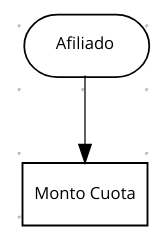
\includegraphics[width=3cm]{drools_diagram.png}
	\end{figure}
\end{center}

\begin{center}
	\begin{figure}
		\includegraphics*[viewport=0 550 789 1175, width=1.3\textwidth]{drools_table.png}
		\includegraphics*[viewport=0 0 789 550, width=1.3\textwidth]{drools_table.png}
	\end{figure}
\end{center}

\paragraph{Gestión de reglas.}
Drools provee un editor visual para la edición de reglas que utilizan \acrshort{dmn}. El editor es una librería web autocontenida, también existe una extensión para Visual Studio Code, que expone la funcionalidad de la misma.

\paragraph{Integración.}
Las reglas de Drools pueden hacer uso de \acrcomplete{pojo}, es decir objetos con campos, getters, setters y constructores, funcionalidad que no pudo ser utilizada en el ejemplo por los problemas mencionados en \cref{para:drools_mantenimiento}.

Alternativamente, los tipos pueden ser definidos utilizando en el editor visual, pasando luego mapas con los valores correspondientes, siendo las claves los nombres de los campos.

\paragraph{Mantenimiento.}\label{para:drools_mantenimiento}
Este motor de reglas es open source y de uso libre, y su desarrollo continúa actualmente activo (hasta la última fecha de edición de esta sección, 20/03/25, la última versión fue publicada el 28/04/24).

Utilizando Ubuntu 22.04.5 LTS, tanto en la extensión como la librería web, se notaron problemas a la hora de importar de otros modelos o de clases Java. Los archivos \verb|.dmn| no eran encontrados por la extensión, mientras que la opción para importar clases Java no estaba disponible. Por otro lado, al cambiar los tipos de las expresiones (Feel Expresion en el ejemplo arriba) al finalizar la edición de uno, los otros volvía a tener el valor inicial de <Undefined>, que es la razón de que tengan ese valor en el ejemplo anterior.

Adicionalmente, incluyendo la librería en un sitio web, únicamente instanciando el componente editor de la librería resulta en numerosos mensajes de advertencia en la consola.

\section{\href{https://openl-tablets.org/}{OpenL Tablets}}
OpenL Tablets es un sistema de gestión de reglas y un motor de reglas basado en la representación de reglas como tablas, desarrollado por el \href{https://openl-tablets.org/community/team}{equipo de OpenL}. Su desarrollo comenzó en 2003 como un projecto interno y fue luego publicado en 2006 en SourceForge. En un principio era únicamente un motor de reglas, convirtiendose en un sistema de gestión de reglas a partir de la versión 5.

\paragraph{Expresividad.}
Para la definición de las reglas se utilizan tablas basadas en Microsoft Excel. Dentro de estas celdas pueden haver valores, acciones o expressiones. Las últimas dos hacen uso de BEX, que es una extensión de la gramática de Java.

\begin{table}[!ht]
	\makeatletter\@ifundefined{tablewidth}{\newlength{\tablewidth}}{}
\makeatother\setlength{\tablewidth}{\dimexpr \textwidth - 3\arrayrulewidth - 6\tabcolsep \relax}
\setlength{\extrarowheight}{-5pt}

\begin{tabular}{|p{0.21\tablewidth}|p{0.27\tablewidth}|p{0.51\tablewidth}|}
		\hline
		\multicolumn{3}{|C{{\dimexpr 1.0\tablewidth + 2\arrayrulewidth + 4\tabcolsep \relax}}|}{\color[HTML]{FFFFFF}\cellcolor[HTML]{000000}Rules Double CalcularCuota(AfiliacionWrapper afiliado)} \\ \hline
		\color[HTML]{000000}\cellcolor[HTML]{CCFFFF}C1
		 & \color[HTML]{000000}\cellcolor[HTML]{CCFFFF}C2
		 & \color[HTML]{000000}\cellcolor[HTML]{CCFFFF}RET1                                                                                                                                         \\ \hline
		\color[HTML]{000000}\cellcolor[HTML]{CCFFFF}categoria
		 & \color[HTML]{000000}\cellcolor[HTML]{CCFFFF}subcategoria
		 & \color[HTML]{000000}\cellcolor[HTML]{CCFFFF}value                                                                                                                                        \\ \hline
		\cellcolor[HTML]{CCFFFF}
		 & \cellcolor[HTML]{CCFFFF}
		 & \color[HTML]{000000}\cellcolor[HTML]{CCFFFF}Double value                                                                                                                                 \\ \hline
		\color[HTML]{000000}\cellcolor[HTML]{FFFF99}Categoria
		 & \color[HTML]{000000}\cellcolor[HTML]{FFFF99}Sub Categoria
		 & \color[HTML]{000000}\cellcolor[HTML]{FFCC99}Fee Value                                                                                                                                    \\ \hline
		\cellcolor[HTML]{FFFF99}
		 & \color[HTML]{000000}\cellcolor[HTML]{FFFF99}CONYUGE
		 & \color[HTML]{000000}\cellcolor[HTML]{FFCC99}=CalcularCuota(conyuge) * 0.7\strut                                                                                                          \\\cline{2-3} \noalign{\vskip 0.5pt}
		\multirow{-2}{0.21\tablewidth}{\color[HTML]{000000}\cellcolor[HTML]{FFFF99}FAMILIAR}
		 & \color[HTML]{000000}\cellcolor[HTML]{FFFF99}DESCENDIENTE\allowbreak\_PRIMER\allowbreak\_GRADO
		 & \color[HTML]{000000}\cellcolor[HTML]{FFCC99}0                                                                                                                                            \\ \hline
		\cellcolor[HTML]{FFFF99}
		 & \color[HTML]{000000}\cellcolor[HTML]{FFFF99}BECARIO
		 & \color[HTML]{000000}\cellcolor[HTML]{FFCC99}=CMMU * ModificadorBecario(afiliado)\strut                                                                                                   \\\cline{2-3} \noalign{\vskip 0.5pt}
		\multirow{-2}{0.21\tablewidth}{\color[HTML]{000000}\cellcolor[HTML]{FFFF99}VOLUNTARIO\allowbreak\_ADHERENTE}
		 & \color[HTML]{000000}\cellcolor[HTML]{FFFF99}AGENTE\allowbreak\_UNSL\allowbreak\_CON\allowbreak\_LICENCIA
		 & \color[HTML]{000000}\cellcolor[HTML]{FFCC99}=afiliado.getHaberPercibido() * ModificadorAgente(afiliado)                                                                                  \\ \hline
		\cellcolor[HTML]{FFFF99}
		 & \cellcolor[HTML]{FFFF99}
		 & \color[HTML]{000000}\cellcolor[HTML]{FFCC99}=error(``categoria desconocida'')                                                                                                            \\ \hline
	\end{tabular}

	\caption{Tabla principal del ejemplo}
\end{table}

\begin{table}[!ht]
	\makeatletter\@ifundefined{tablewidth}{\newlength{\tablewidth}}{}
\makeatother\setlength{\tablewidth}{\dimexpr \textwidth - 2\arrayrulewidth - 4\tabcolsep \relax}
\setlength{\extrarowheight}{-5pt}

\begin{tabular}{|p{0.33\tablewidth}|p{0.67\tablewidth}|}
	\hline
	\multicolumn{2}{|C{{\dimexpr 1.0\tablewidth + 1\arrayrulewidth + 2\tabcolsep \relax}}|}{\color[HTML]{FFFFFF}\cellcolor[HTML]{000000}Environment} \\ \hline
	\color[HTML]{000000}\cellcolor[HTML]{FFFF99}import
	 & \color[HTML]{000000}\cellcolor[HTML]{FFFF99}com.example.afiliacion\allowbreak\_wrapper                                                        \\ \hline
\end{tabular}

	\caption{Importación de las clases de Java}
	\label{tab:openl_java_import}
\end{table}

\begin{table}[!ht]
	\makeatletter\@ifundefined{tablewidth}{\newlength{\tablewidth}}{}
\makeatother\setlength{\tablewidth}{\dimexpr \textwidth - 3\arrayrulewidth - 6\tabcolsep \relax}
\setlength{\extrarowheight}{-5pt}

\begin{tabular}{|p{0.28\tablewidth}|p{0.25\tablewidth}|p{0.47\tablewidth}|}
	\hline
	\multicolumn{3}{|C{{\dimexpr 1.0\tablewidth + 2\arrayrulewidth + 4\tabcolsep \relax}}|}{\color[HTML]{FFFFFF}\cellcolor[HTML]{000000}Rules Double ModificadorBecario(AfiliacionWrapper afiliado)} \\ \hline
	\multicolumn{2}{|C{{\dimexpr 0.5330525030525031\tablewidth + 1\arrayrulewidth + 2\tabcolsep \relax}}|}{\color[HTML]{000000}\cellcolor[HTML]{CCFFFF}C3}
	 & \color[HTML]{000000}\cellcolor[HTML]{CCFFFF}RET1                                                                                                                                              \\ \hline
	\multicolumn{2}{|C{{\dimexpr 0.5330525030525031\tablewidth + 1\arrayrulewidth + 2\tabcolsep \relax}}|}{\color[HTML]{000000}\cellcolor[HTML]{CCFFFF}edad}
	 & \color[HTML]{000000}\cellcolor[HTML]{CCFFFF}value                                                                                                                                             \\ \hline
	\color[HTML]{000000}\cellcolor[HTML]{CCFFFF}int min
	 & \color[HTML]{000000}\cellcolor[HTML]{CCFFFF}int max
	 & \color[HTML]{000000}\cellcolor[HTML]{CCFFFF}Double value                                                                                                                                      \\ \hline
	\color[HTML]{000000}\cellcolor[HTML]{FFFF99}Desde
	 & \color[HTML]{000000}\cellcolor[HTML]{FFFF99}Hasta
	 & \color[HTML]{000000}\cellcolor[HTML]{FFCC99}Modificador                                                                                                                                       \\ \hline
	\cellcolor[HTML]{FFFF99}
	 & \color[HTML]{000000}\cellcolor[HTML]{FFFF99}30
	 & \color[HTML]{000000}\cellcolor[HTML]{FFCC99}0.45                                                                                                                                              \\ \hline
	\color[HTML]{000000}\cellcolor[HTML]{FFFF99}31
	 & \color[HTML]{000000}\cellcolor[HTML]{FFFF99}45
	 & \color[HTML]{000000}\cellcolor[HTML]{FFCC99}0.82                                                                                                                                              \\ \hline
	\color[HTML]{000000}\cellcolor[HTML]{FFFF99}46
	 & \color[HTML]{000000}\cellcolor[HTML]{FFFF99}55
	 & \color[HTML]{000000}\cellcolor[HTML]{FFCC99}1                                                                                                                                                 \\ \hline
	\color[HTML]{000000}\cellcolor[HTML]{FFFF99}56
	 & \color[HTML]{000000}\cellcolor[HTML]{FFFF99}65
	 & \color[HTML]{000000}\cellcolor[HTML]{FFCC99}1.2                                                                                                                                               \\ \hline
	\color[HTML]{000000}\cellcolor[HTML]{FFFF99}66
	 & \cellcolor[HTML]{FFFF99}
	 & \color[HTML]{000000}\cellcolor[HTML]{FFCC99}2                                                                                                                                                 \\ \hline
\end{tabular}

	\caption{Tabla modificador becario}
\end{table}

\begin{table}[!ht]
	\makeatletter\@ifundefined{tablewidth}{\newlength{\tablewidth}}{}
\makeatother\setlength{\tablewidth}{\dimexpr \textwidth - 3\arrayrulewidth - 6\tabcolsep \relax}
\setlength{\extrarowheight}{-5pt}

\begin{tabular}{|p{0.23\tablewidth}|p{0.24\tablewidth}|p{0.53\tablewidth}|}
	\hline
	\multicolumn{3}{|C{{\dimexpr 0.9999999999999999\tablewidth + 2\arrayrulewidth + 4\tabcolsep \relax}}|}{\color[HTML]{FFFFFF}\cellcolor[HTML]{000000}Rules Double ModificadorAgente(AfiliacionWrapper afiliado)} \\ \hline
	\multicolumn{2}{|C{{\dimexpr 0.4692429792429792\tablewidth + 1\arrayrulewidth + 2\tabcolsep \relax}}|}{\color[HTML]{000000}\cellcolor[HTML]{CCFFFF}C3}
	 & \color[HTML]{000000}\cellcolor[HTML]{CCFFFF}RET1                                                                                                                                                            \\ \hline
	\multicolumn{2}{|C{{\dimexpr 0.4692429792429792\tablewidth + 1\arrayrulewidth + 2\tabcolsep \relax}}|}{\color[HTML]{000000}\cellcolor[HTML]{CCFFFF}edad}
	 & \color[HTML]{000000}\cellcolor[HTML]{CCFFFF}value                                                                                                                                                           \\ \hline
	\color[HTML]{000000}\cellcolor[HTML]{CCFFFF}int min
	 & \color[HTML]{000000}\cellcolor[HTML]{CCFFFF}int max
	 & \color[HTML]{000000}\cellcolor[HTML]{CCFFFF}Double value                                                                                                                                                    \\ \hline
	\color[HTML]{000000}\cellcolor[HTML]{FFFF99}Desde
	 & \color[HTML]{000000}\cellcolor[HTML]{FFFF99}Hasta
	 & \color[HTML]{000000}\cellcolor[HTML]{FFCC99}Modificador                                                                                                                                                     \\ \hline
	\cellcolor[HTML]{FFFF99}
	 & \color[HTML]{000000}\cellcolor[HTML]{FFFF99}30
	 & \color[HTML]{000000}\cellcolor[HTML]{FFCC99}0.4                                                                                                                                                             \\ \hline
	\color[HTML]{000000}\cellcolor[HTML]{FFFF99}31
	 & \color[HTML]{000000}\cellcolor[HTML]{FFFF99}45
	 & \color[HTML]{000000}\cellcolor[HTML]{FFCC99}0.78                                                                                                                                                            \\ \hline
	\color[HTML]{000000}\cellcolor[HTML]{FFFF99}46
	 & \color[HTML]{000000}\cellcolor[HTML]{FFFF99}55
	 & \color[HTML]{000000}\cellcolor[HTML]{FFCC99}0.95                                                                                                                                                            \\ \hline
	\color[HTML]{000000}\cellcolor[HTML]{FFFF99}56
	 & \color[HTML]{000000}\cellcolor[HTML]{FFFF99}65
	 & \color[HTML]{000000}\cellcolor[HTML]{FFCC99}1.13                                                                                                                                                            \\ \hline
	\color[HTML]{000000}\cellcolor[HTML]{FFFF99}66
	 & \cellcolor[HTML]{FFFF99}
	 & \color[HTML]{000000}\cellcolor[HTML]{FFCC99}1.86                                                                                                                                                            \\ \hline
\end{tabular}

	\caption{Tabla secundaria modificador agente UNSL}
\end{table}

\paragraph{Gestión de reglas.}
El motor posee una aplicación web para la creación, modificación, eliminación, prueba y versionado. Además, se separan los repositorios de diseño y producción, permitiendo la colaboración en edición de reglas y el versionado de las mismas de forma independiente del \acrshort{si}. Alternativamente, pueden utilizarse Microsoft Excel, of software similar como Libre Office, para la creación, modificación y eliminación de las reglas.

\paragraph{Integración.}
Por otra parte, OpenL Tablets posee otra aplicación para exponer las reglas almacenadas en un repositorio como servicios web. Alternativamente, brinda clases de utilidad para la compilación de las reglas. Estas utilizan las tablas para generar clases wrapper, las cuales también pueden ser específicadas manualmente. En caso de utilzar las clases generadas, las reglas pueden accederse por medio de la reflección, siendo métodos de las clases con los mismos nombres de las reglas.

Las reglas de OpenL pueden hacer uso directo de las instancias de las clases Java. Para esto, se utiliza una tabla para importar las mismas, como la presente en \cref{tab:openl_java_import}.

\paragraph{Mantenimiento.}
Este motor de reglas es open source y de uso libre, y su desarrollo continúa actualmente activo (hasta la última fecha de edición de esta sección, 20/03/25, la última versión fue publicada el 28/02/2025).



\chapter{Relevamiento código fuente}


\chapter{Traducción al paradigma funcional}

\section{Caso de estudio 1}

\desarrollar[inline]{Toma el ejemplo más simple desarrollado y explicas como lo pasaste a funcional}

\section{Caso de estudio 2}

\section{Caso de estudio 3}

\chapter{Parametrización en reglas}
\label{chap:solucion}

\section{Elección del Motor a Utilizar}
Como se mencionó anteriormente, el objectivo de este trabajo es facilitar la gestión de las reglas de un \SIOSU, particularmente por personas sin o con reducidos conocimientos relacionados con la programación. Teniendo esto en cuenta, se considera que, irrespectivamente de los demás aspectos considerados en el criterio de decisión, Drools y OpenL Tablets resultan las únicas opciones de interés para este trabajo. La siguiente es una comparación más detallada de estas opciones:

\paragraph{Expresividad.}
La expresividad que ambos proveen para las reglas resulta comparable. Dicho esto, las tablas de Excel probablemente resulten más familiares para la mayoría de personas que los diagramas DMN.

\paragraph{Gestión de reglas.}
En este aspecto, OpenL Tablets resulta superior, ya que cuenta con herramientas para el versionado de las reglas, además del resto de capacidades que comparte con Drools, como la creación, modificación y eliminación de reglas.

\paragraph{Integración.}
En este campo los motores son similares, por lo menos en su especificación. Dados los problemas mencionados en la subsección de Drools del cápitulo anterior, estás capacidades no pudieron ser probadas para este.

\paragraph{Mantenimiento.}
Ambos proyectos son actualemente (hasta la última fecha de edición de esta sección, 08/04/2025) mantenidos.

Por otra parte, mientras que en el caso de OpenL Tablets no se encontró ningún problema durante la elaboración del ejemplo, lo mismo no se puede decir de Drools. Con este último se encontraron varios problemas, mencionados en la sección correspondiente del cápitulo anterior, relacionados con las herramientas para la creación y edición de las reglas.

\paragraph{Elección final.}
Teniendo en cuenta este análisis, se puede ver que, en los aspectos que resultan de interés para este trabajo, OpenL Tablets resulta igual o superior en cada uno. Consecuentemente, se hará uso del mismo de aquí en adelante.

\section{Caso de estudio 1}

\desarrollar[inline]{Toma el ejemplo más simple desarrollado y explicas como lo parametrizaste con el motor de reglas.}


\section{Caso de estudio 2}

\section{Caso de estudio 3}

\chapter{Conclusiones}

\backmatter

\printbibliography

\end{document}
